\chapter{Einführung}
    \label{chapter:introduction}
    Ein zeitgemäßer Internetauftritt mit aktuellen Inhalten
    ist ein wichtiger Bestandteil der Öffentlichkeitsarbeit jeder Organisation,
    da sie für viele Interessierte die erste Anlaufstelle zur Beschaffung von Informationen ist.
    Wichtige Gründe hierfür sind die ständige Verfügbarkeit sowie die Orts-
    und Geräteunabhängigkeit.
    Eine Webseite steht zu jeder Tageszeit zur Verfügung und kann
    dank moderner Endgeräte wie Smartphones und Tablets
    auch unterwegs aufgerufen werden.
    Für den Nutzer stellt der Internetauftritt deshalb ein Medium dar,
    das er einfach, spontan und flexibel verwenden kann.
    Wegen dieser Beliebtheit dient die Webseite neben der reinen Bereitstellung von Informationen
    auch der eigenen Werbung und Vermarktung und spielt eine wichtige Rolle im Erfolg einer Organisation.
    Zwei Eigenschaften des Webauftrittes sind laut \citet{sillence:onlineHealthSites} dabei
    entscheidend: Inhalt und Design.
    Jede Organisation ist deshalb angehalten, laufend ihre Webseite inhaltlich zu pflegen
    und ihr regelmäßig ein modernes Design zu geben.
    Andernfalls läuft sie Gefahr die Erwartungen ihrer Besucher nicht zu erfüllen,
    die sich deshalb schlecht angesprochen fühlen und womöglich zur Konkurrenz wechseln.

    Eine Modernisierung des Designs stellt den Inhaber der Webseite zwangsläufig vor die Frage,
    was mit seinen bestehenden Inhalten geschehen soll.
    Die \fernUni\footnote{\url{http://www.fernuni-hagen.de/}}
    steht vor einer solchen Umstellung ihres Internetauftrittes,
    wodurch die Seite unter anderem ein responsives Design erhält und damit besser für
    mobile Endgeräte geeignet sein wird.
    Viele Inhalte möchte die Universität nicht nur übernehmen,
    sondern auch in ein anderes \gls{cms} migrieren.
    Im Folgenden werden die Herausforderungen bei diesem Vorhaben erläutert,
    aus der sich anschließend das Thema dieser Arbeit ergibt.

    \section{Die CMS-Migration der \fernUni}
        \label{section:fernUniChallenges}
        An der {\fernUni} arbeiten {\editors} mit dem \gls{cms} \textit{{\imperia} 9}
        \cite{fernUni:imperia}
        der \textit{pirobase imperia GmbH}\footnote{https://www.pirobase-imperia.com}.
        Eine Ausnahme stellt allerdings die Fakultät für \gls{ksw} dar.
        Hier ist das Open-Source-Produkt \textit{\wordpress}\footnote{https://wordpress.org/} im Einsatz.
        Für die Fakultät ist ein Vorteil dieser Abspaltung,
        dass sie frei über das Design ihrer Seiten bestimmen kann
        und deshalb schon jetzt ein responsives Design verwendet.
        Für die Universität als Ganzes hat dies allerdings unter anderem folgende Nachteile:

        \begin{enumerate}
            \item   Es existiert kein durchgehendes Corporate Design.
            \item   Es existiert keine zentrale Datenhaltung, da beide Systeme ihre Inhalte getrennt speichern.
                    Redundanzen sind nicht auszuschließen.
            \item   Es entsteht ein erhöhter Administrationsaufwand.
            \item   {\editors} arbeiten mit verschiedenen Systemen und müssen entsprechend geschult sein.
        \end{enumerate}

        Diese negativen Auswirkungen 
        begründen die Entscheidung, dass die Seiten der Fakultät \gls{ksw}
        in Zukunft ebenfalls das neue gemeinsame Design der {\fernUni} verwenden und
        über {\imperia} gepflegt werden.
        Vorhandene Inhalte möchte die Fakultät übernehmen,
        sodass eine Migration von {\wordpress} zu {\imperia} notwendig ist.
        Es folgen die Herausforderungen, die diese Migration birgt.

        \paragraph{Unterschiedliche Strukturierung der Inhalte}
        Vergleicht man die Eingabemasken zur Inhaltspflege beider Systeme, fällt auf,
        dass sie unterschiedlichen Herangehensweisen folgen.
        Abbildung \ref{image:introductionFernUniImperiaForm} zeigt dazu ein Formular
        zur Pflege eines Mitarbeiters in {\imperia}.

        \begin{figure}[htb]
            \centering
            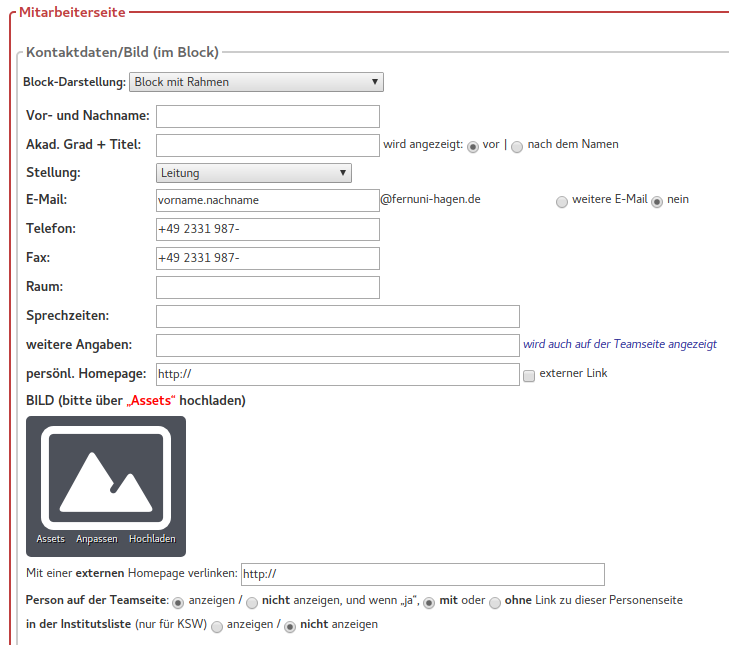
\includegraphics[width=0.7\textwidth]{../resources/imperia/team.png}
            \caption{Eingabemaske zur Pflege eines Mitarbeiters in {\imperia}}
            \label{image:introductionFernUniImperiaForm}
        \end{figure}

        Die Eingabemaske besteht aus einem feingranularen Formular,
        welches für verschiedene Angaben des Mitarbeiters unterschiedliche Formularfelder
        vorsieht.
        Abbildung \ref{image:introductionFernUniWordpressForm} zeigt,
        wie Mitarbeiter in {\wordpress} gepflegt werden.

        \begin{figure}[htb]
            \centering
            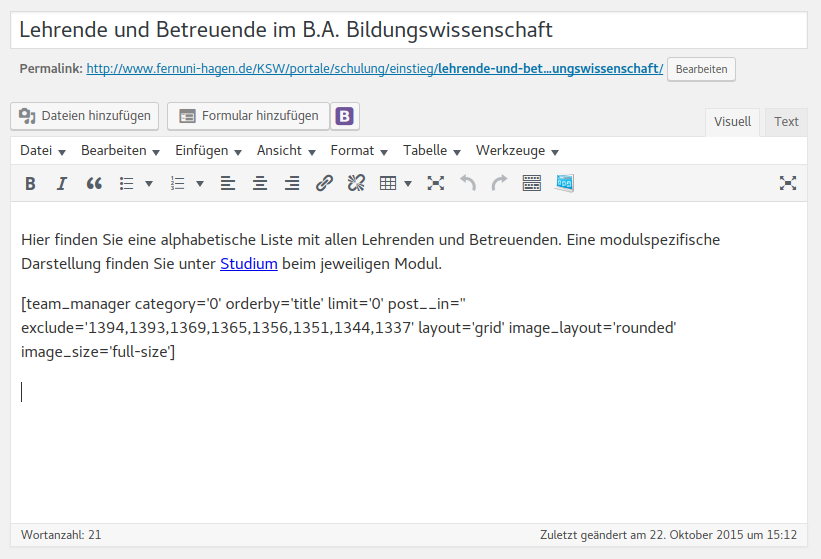
\includegraphics[width=0.7\textwidth]{../resources/wordpress/teachers.png}
            \caption{Eingabemaske zur Pflege eines Mitarbeiters in {\wordpress}}
            \label{image:introductionFernUniWordpressForm}
        \end{figure}
        
        Hier besteht das Formular lediglich aus zwei Feldern:
        eines für den Titel der Seite und eines für den Inhalt der Seite.
        Die Angaben eines Mitarbeiters werden unstrukturiert in das zweite Feld eingegeben.
        Für eine Migration stehen generell zwei Möglichkeiten zur Auswahl,
        um mit dieser Differenz umzugehen:

        \begin{enumerate}
            \item   Für die aus {\wordpress} stammenden Seiten werden in {\imperia} Formulare geschaffen,
                    die ebenfalls nur Felder für den Titel und den Inhalt einer Seite enthalten.
                    Die Inhalte können dann 1:1 übertragen werden.
            \item   Die Inhalte der aus {\wordpress} stammenden Seiten werden vor der Migration strukturiert,
                    sodass sie in die feingranularen Formulare in {\imperia} übertragen werden können.
        \end{enumerate}

        Beide Ansätze besitzen Vor- und Nachteile.
        Die erste Methode ist vergleichsweise einfach zu realisieren,
        hätte allerdings zur Folge, dass für die Inhalte der Fakultät \gls{ksw} Sonderbehandlungen
        in {\imperia} geschaffen werden, da die restlichen Fakultäten ihre bekannten feingranularen
        Formulare beibehalten möchten.
        Das hieße zum Beispiel, dass die Fakultät \gls{ksw} andere Formulare für die Pflege aktueller
        Nachrichten verwendet, als die restlichen Fakultäten.
        Da das Design beider Seiten am Ende aber identisch sein soll, bedeuten unterschiedliche Formulare
        auch Sonderbehandlungen in der Erzeugung der Seiten.
        Solche Sonderbehandlungen erzeugen erhöhte Aufwände sowohl im initialen Modernisierungsprojekt
        als auch in der späteren Wartung.
        Nicht auszuschließen ist außerdem, dass {\editors} der Fakultät \gls{ksw} aufgrund der groben Formularstruktur
        weniger redaktionelle Möglichkeiten hätten, als die anderer Fakultäten.

        Die Vor- und Nachteile der zweiten Methode sind komplementär zu denen der ersten Methode.
        Das Resultat ihrer Umsetzung wären universitätsweit einheitliche Formulare
        ohne Sonderbehandlungen für die ehemaligen Seiten aus {\wordpress}.
        Gleichzeitig ist die Strukturierung der Inhalte aber keine triviale Aufgabe.
        Unter anderem stellen sich dabei die folgenden Fragen:

        \begin{itemize}
            \item Welche Arten von Seiten liegen vor (Aktuelle Nachrichten, Prüfungen, Module, etc.)?
            \item Welche Inhalte besitzen diese Seitentypen?
            \item Wie müssen diese Inhalte strukturiert werden?
        \end{itemize}

        Die Beantwortung dieser Fragen erfordert eine genaue Analyse der Seiten der Fakultät \gls{ksw}
        und einen Vergleich mit den geplanten Seiten und Formularen in {\imperia}.
        
        \paragraph{Dynamisch generierte Inhalte}
        Nicht alle Inhalte werden in {\wordpress} statisch in einer Datenbank vorgehalten.
        Oftmals werden Teile dynamisch beim Aufruf einer Webseite
        generiert\footnote{vgl. Kapitel \ref{section:WordPress}}.
        Ein Beispiel zeigt Abbildung \ref{image:introductionFernUniWordpressOverviewForm},
        in dem alle Mitarbeiter eines Lehrgebietes auf einer Übersichtsseite eingebunden werden.

        \begin{figure}[htb]
            \centering
            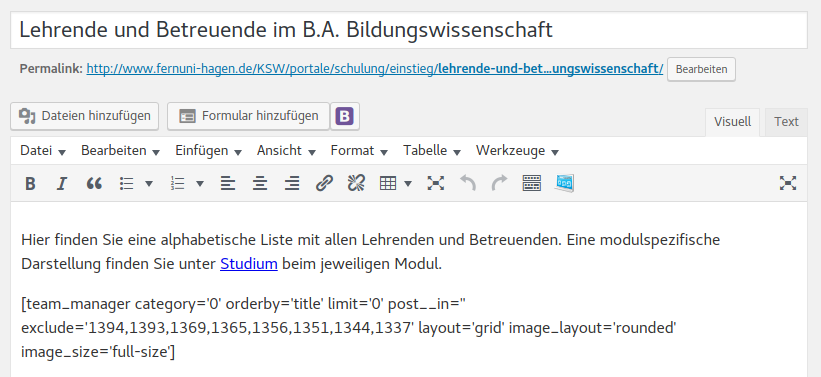
\includegraphics[width=0.7\textwidth]{../resources/wordpress/teachers-overview.png}
            \caption{Übersichtsseite aller Mitarbeiter in {\wordpress}}
            \label{image:introductionFernUniWordpressOverviewForm}
        \end{figure}

        Eine Migration zu {\imperia} muss dies berücksichtigen und entsprechendes {\wordpress}-Markup
        geeignet übersetzen oder auswerten.

        \paragraph{Aufwand}
        Die Durchführung einer Migration erzeugt auch nennenswerte operative Aufwände.
        Die Inhalte jeder einzelnen Seite der Fakultät \gls{ksw} müssen
        mit den neuen Strukturen abgeglichen und in diese überführt werden.
        Bei den über 4000 Seiten der Fakultät
        würde sich diese Aufgabe ohne Automatisierung als bedenklich und anfällig für Fehler erweisen.

    \section{Inhalt und Aufbau der Arbeit}
        Die beschriebenen Herausforderungen
        werfen die Frage auf, wie mittels Software die Inhalte aller Webseiten der Fakultät \gls{ksw}
        automatisch in definierte Strukturen überführt werden können.
        Ausgehend von dieser konkreten Anforderung der {\fernUni} stellt diese Arbeit eine
        \gls{dsl} vor, die zur Instrumentierung eines Softwaresystems dient,
        welches die Inhalte der Seiten einer
        Website\footnote{vgl. Kapitel \ref{section:problemAnalysisWebpagesInTheWWW}}
        automatisch klassifiziert.
        Dieses System ist ebenfalls Teil dieser Arbeit.

        Im folgenden Kapitel \ref{chapter:ProblemAnalysis} wird die Problemstellung ausführlicher
        analysiert und spezifiziert, was auch die Betrachtung der Problemdomäne beinhaltet.
        Aufbauend auf den dann vorliegenden Erkenntnissen erarbeitet
        Kapitel \ref{chapter:SolutionConcept}
        ein Lösungskonzept und erläutert die Architektur des Systems.
        Eine detaillierte Betrachtung der einzelnen Komponenten des Systems
        erfolgt in Kapitel \ref{chapter:SolutionDetails}.
        Dazu geht das Kapitel auf die Anforderungen an jede Komponente,
        konzeptionelle Details, Schnittstellen sowie Aspekte der Implementierung ein.       
        In Kapitel \ref{chapter:Findings} findet das System in zwei Fallbeispielen der {\fernUni}
        Anwendung, deren Ergebnisse präsentiert werden.
        Eine kritische Diskussion dieser Ergebnisse erfolgt anschließend in
        Kapitel \ref{chapter:FindingsDiscussion}.
        Abschließend fasst Kapitel \ref{chapter:SummaryAndOutlook}
        diese Arbeit zusammen und zeigt Erweiterungsmöglichkeiten
        des vorgestellten Systems auf.

        Einige Kapitel dieser Arbeit setzen gewisse Kenntnisse voraus.
        Notwendige Grundlagen werden nicht zentral in einem separaten Kapitel vermittelt,
        sondern dort, wo sie benötigt werden.
